\section{高分子}
{\color{red}\begin{center}
        杨雅晴
    \end{center}}
合成聚合物分子是一种由大量单体化学耦合而成的高分子量大分子,聚合物通常是由两个位点的单体连接而成的线性链,且聚合物可分为以下两类:
\begin{itemize}
	\item 均聚物:由N个同种化学类型的单体联结而成的聚合物。(其中,N称为其聚合度)
	\item 共聚物:由两种及以上不同化学类型单体联结而成的聚合物。
\end{itemize}
其中共聚物根据其单体的联结规律不同分为以下两种:
\begin{itemize}
	\item 无规共聚物:共聚物中两结构单元A和B随机出现,其中A和B自身连续的单元数不多,一般在几个到十几个。
	\item 嵌段共聚物:由较长的只有结构单元A的链段和较长的只有结构单元B的链段构成,其中每一链段可达到几百到几千结构单元。
\end{itemize}

%\begin{center}
\begin{figure}[h]
	\centering
	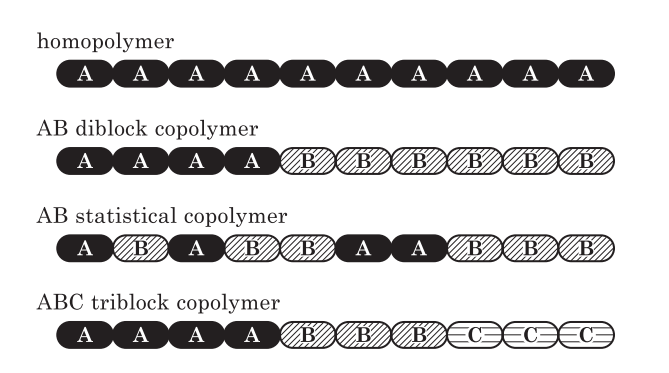
\includegraphics[scale=0.5
    ]{Contents/chapter1/figures/1-1.png}
	\caption{聚合物实例}
\end{figure}
%聚合物实例

\begin{figure}[h]
	\centering
	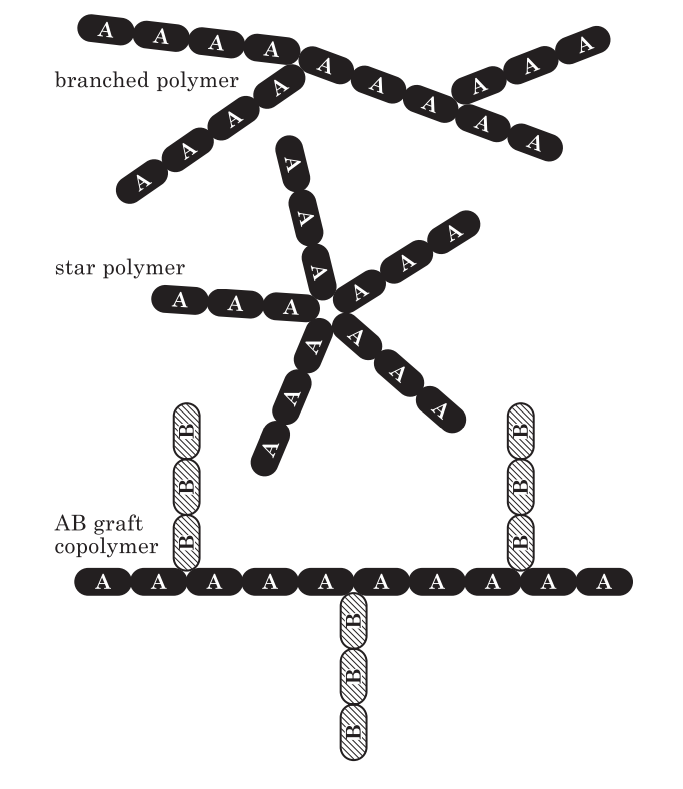
\includegraphics[scale=0.5
	]{Contents/chapter1/figures/1-2.png}
	\caption{聚合物实例}
\end{figure}
%聚合物实例
%\end{center}

\section{建模视角和尺度}

\subsection{介观视角}

解决非均聚合物完全原子化模拟的困难的一种策略为粗粒化原子模型,以便将原子组集中到称为粒子的更大实体中,这些粒子可以不对应于分子种类。粒子间新的有效相互作用势必须重新参数化。我们在最低层面上举例,可以将相邻的原子分组形成粒子,比如将每个$CH_2$单元沿聚乙烯链集中成一个粒子,然后使用经验知识或量子化学计算来拟合描述粒子间成键和非成键相互作用的势函数中的参数。

\begin{figure}[h]
\centering
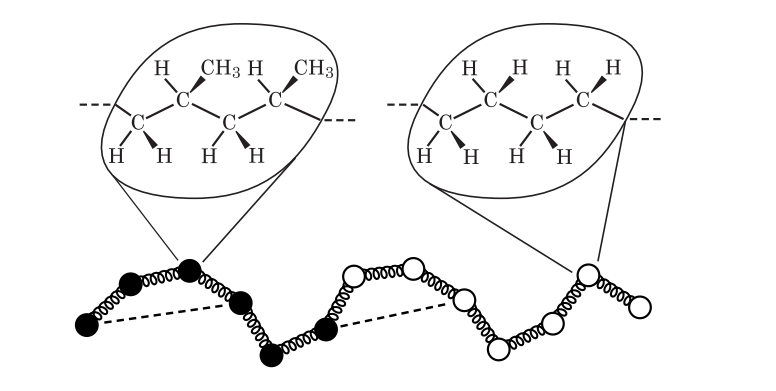
\includegraphics[scale=0.5
]{Contents/chapter1/figures/1-3.png}
\caption{粗粒化模型示例}
\end{figure}

上图为将聚丙烯-聚乙烯嵌段共聚物粗粒化成珠弹簧颗粒模型的原理图。暗珠子表示粗颗粒的聚丙烯颗粒;光珠相当于聚乙烯颗粒。弹簧表示沿聚合物的相邻粒子间的键对势。非成键相互作用(虚线)也出现在这种粗粒度模型中。

恰如聚乙烯、聚丙烯等合成聚合物,我们称骨架上碳碳单键的旋转相对不受阻碍的聚合物为柔性的。这种柔韧性意味着沿着链的特定片段的方向几乎与沿着链移除的10个或更多单体残基的片段的方向无关。一些特殊的合成聚合物和许多生物聚合物,如双链DNA,由于粘结菌株的积累,其硬度和弯曲度要高得多。从而我们有了半柔性或刚性杆聚合物的概念,其决定于聚合物的长度和自由度。本书主要讨论柔性大分子。
